\documentclass{article}
\usepackage{subfig}
\usepackage{placeins}
\usepackage[utf8]{inputenc}

\usepackage{amsfonts}
\usepackage{amssymb}
\usepackage{amsmath}
\usepackage{amsthm}
\usepackage{enumitem}
\usepackage{float}
\usepackage{bm}
\usepackage{graphicx}
\usepackage{color}
\usepackage{hyperref}
\usepackage[margin=3cm]{geometry}
 \usepackage{bbold}

\usepackage{svg}
\begin{document}


% ==============================================================================

\title{\Large{ELEN0062: Project 1 - Report}}
\vspace{1cm}
\author{\small{\bf Stéphane Champailler - s912550 } \\ \small{\bf Christian Fiedler - s204358}}


%\\ \small{\bf Miss Pacman - s222222}}

\maketitle

% ==============================================================================

\def\picwidth{8cm}

\section{Decision tree}
\subsection{Decision boundary and tree depth}
\subsubsection{Decision boundary and tree depth}

When looking at the way the boundary changes with the depth in problem 1 (see figure \ref{boundary1}, we see :
\begin{enumerate}
\item Depth 1 : the boundary shape is too simple to actually represent the data in any meaningful way
\item Depth 2 : The boundary shape fits the red dots quite well, but there are still some blue dots that are classified wrongly.
\item Depth 4 : the boundary classifies most of the points correctly. Which seems normal since a tree of depth 4 can cut the space 4 times, making a 4-sided boundary.
\item Depth 8 and None : the boundary doesn't improve anymore.
\end{enumerate}


When looking at the way the boundary changes with the depth in problem 2 (see figure \ref{boundary2}, we see :
\begin{enumerate}
\item Depth 1 : the boundary shape is too simple to actually represent the data in any meaningful way.
\item Depth 2 : idem
\item Depth 4 : idem
\item Depth 8 : idem
\item Depth None : the boundary is much better but tends to overfit
\end{enumerate}

For the figure 2, overfitting and misclassification are expected. That's because the intersections between the two
ellipses are hard to classify and introduce instabilities.




\begin{figure}[htbp]
  \centering
  
  \subfloat{   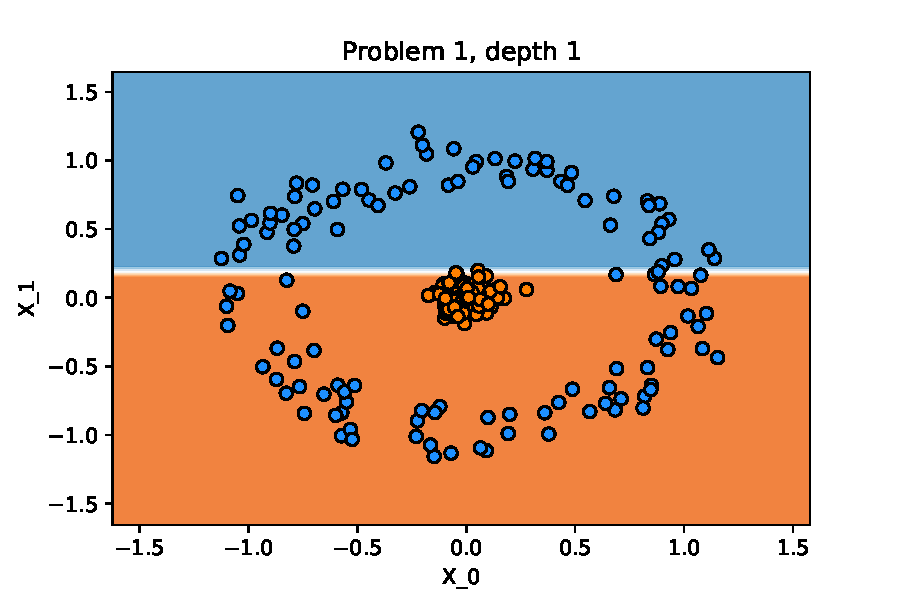
\includegraphics[width=\picwidth]{plots/dec_tree/p1_depth1.pdf}}
  \subfloat{   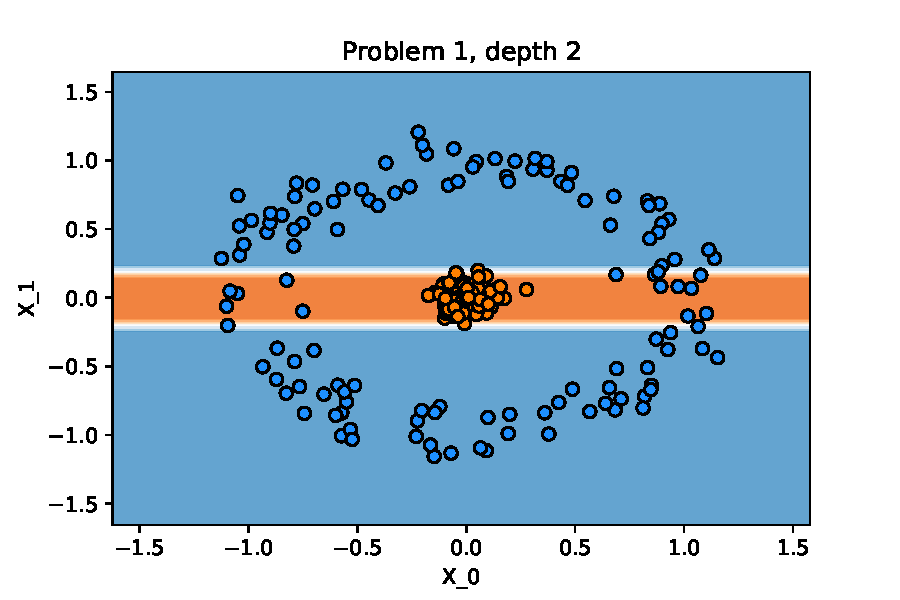
\includegraphics[width=\picwidth]{plots/dec_tree/p1_depth2.pdf}}
  
  \subfloat{   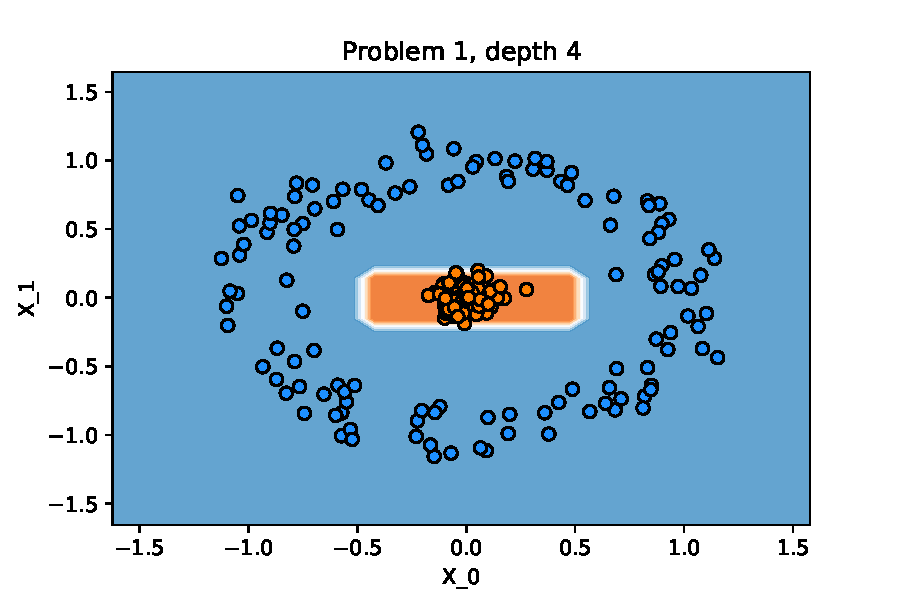
\includegraphics[width=\picwidth]{plots/dec_tree/p1_depth4.pdf}}
  \subfloat{   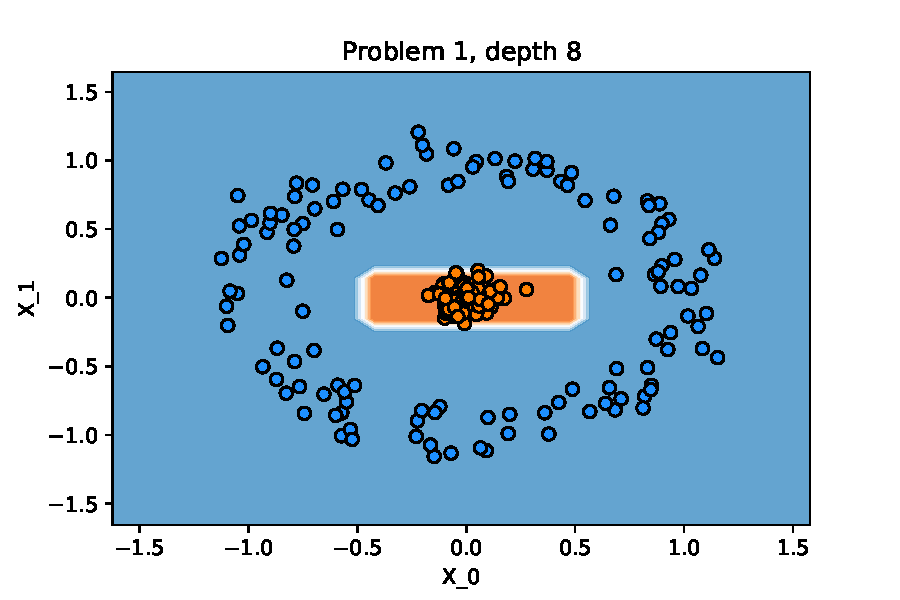
\includegraphics[width=\picwidth]{plots/dec_tree/p1_depth8.pdf}}
  
  \subfloat{   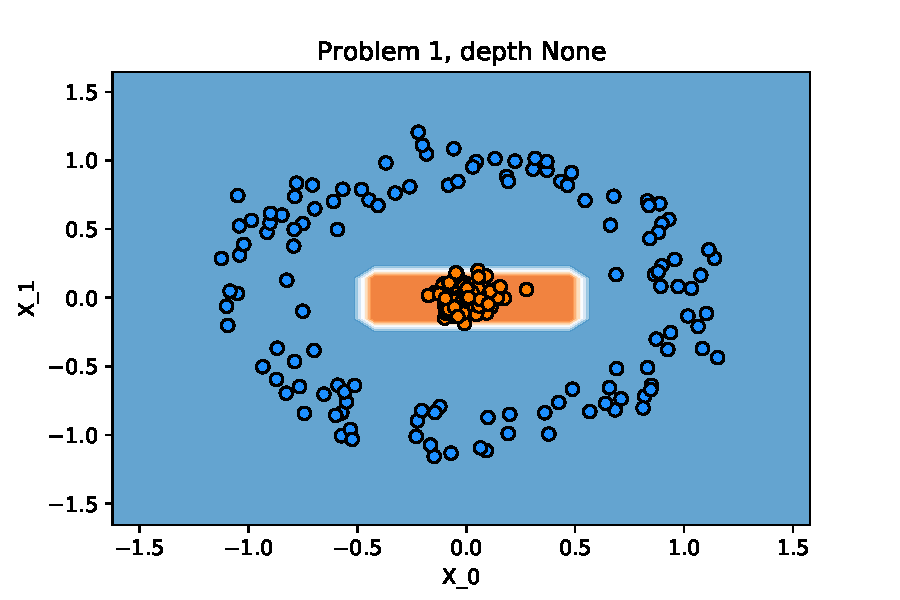
\includegraphics[width=\picwidth]{plots/dec_tree/p1_depthNone.pdf}}
  
  
  \caption{\label{boundary1}Decision boundaries problem 1}
\end{figure}

\begin{figure}[htbp]
  \centering
  \subfloat{ 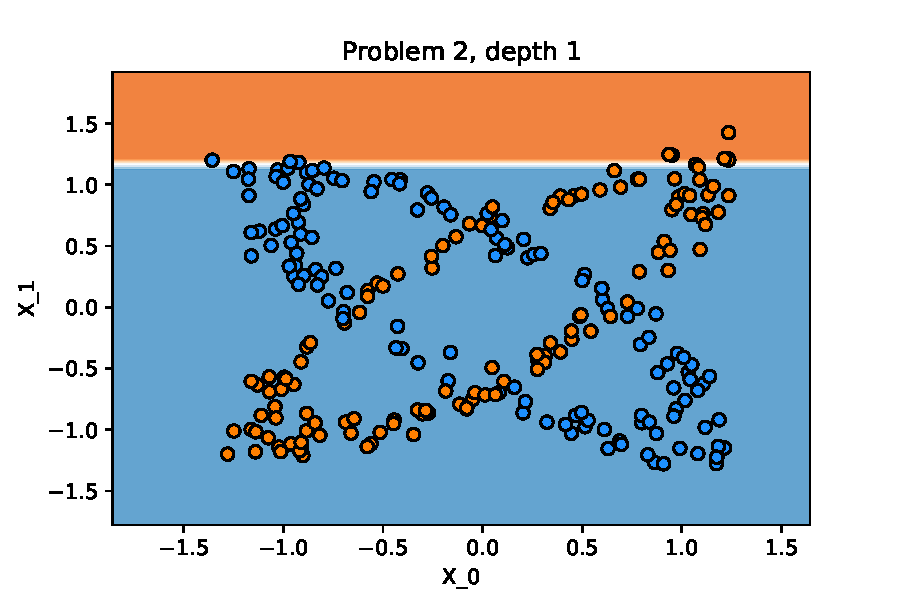
\includegraphics[width=\picwidth]{plots/dec_tree/p2_depth1.pdf}}
  \subfloat{ 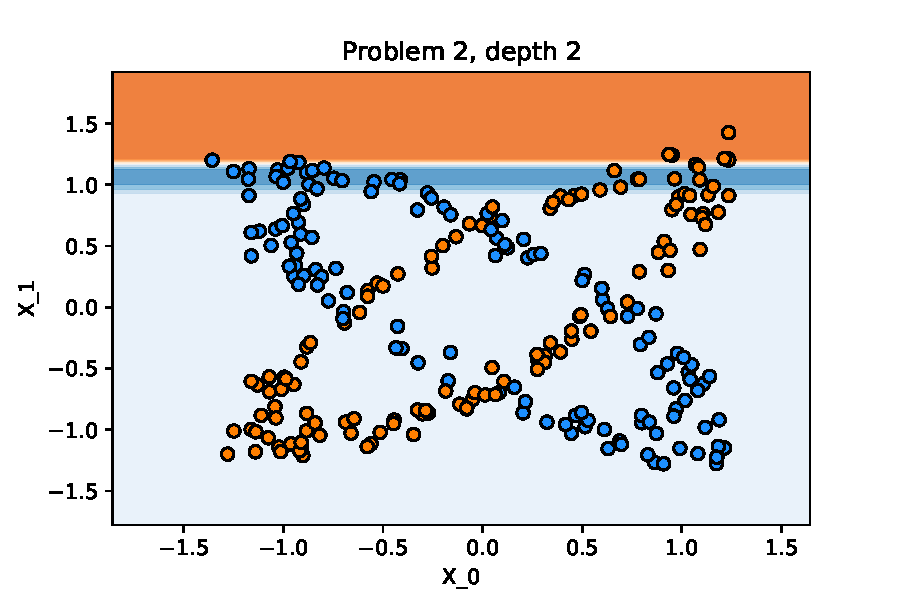
\includegraphics[width=\picwidth]{plots/dec_tree/p2_depth2.pdf}}

  \subfloat{ 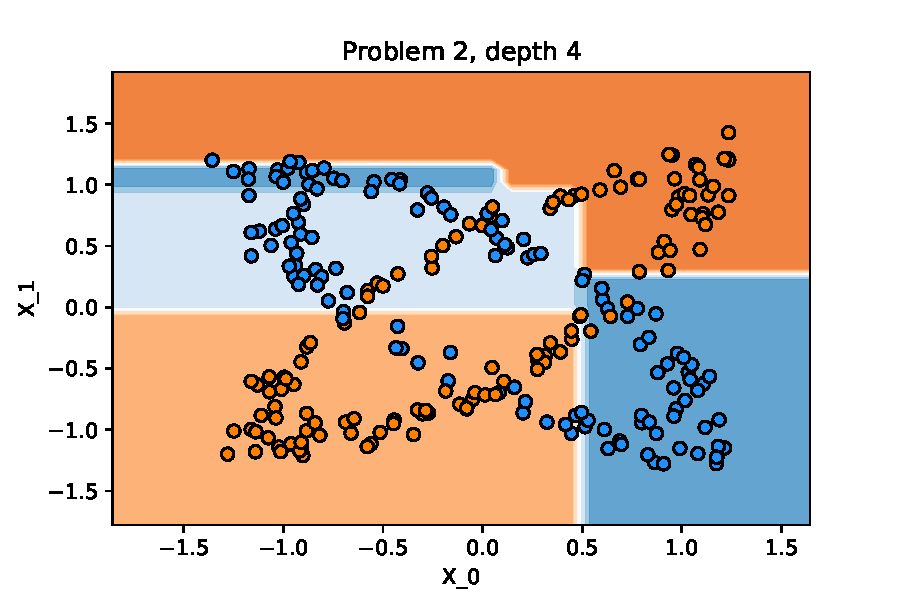
\includegraphics[width=\picwidth]{plots/dec_tree/p2_depth4.pdf}}
  \subfloat{ 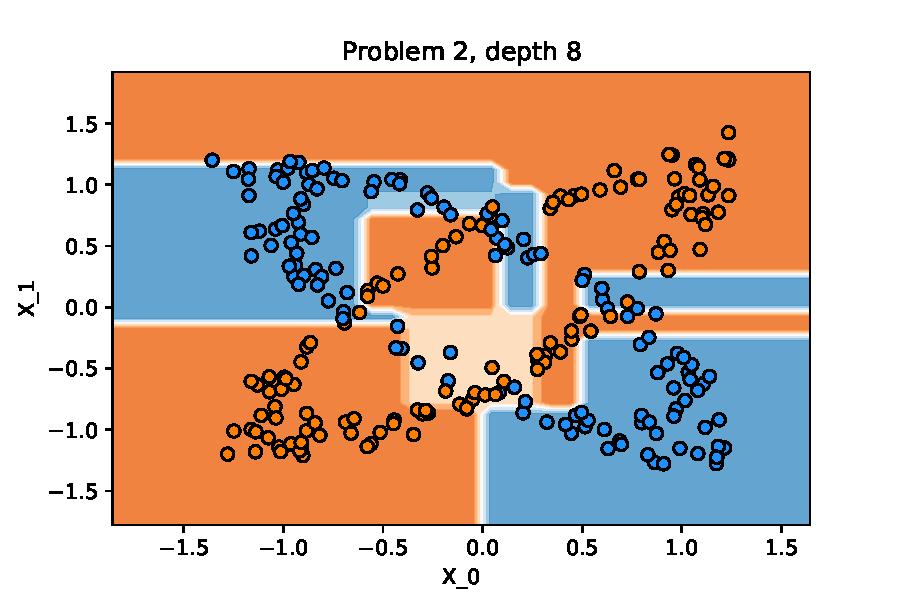
\includegraphics[width=\picwidth]{plots/dec_tree/p2_depth8.pdf}}
  
  \subfloat{ 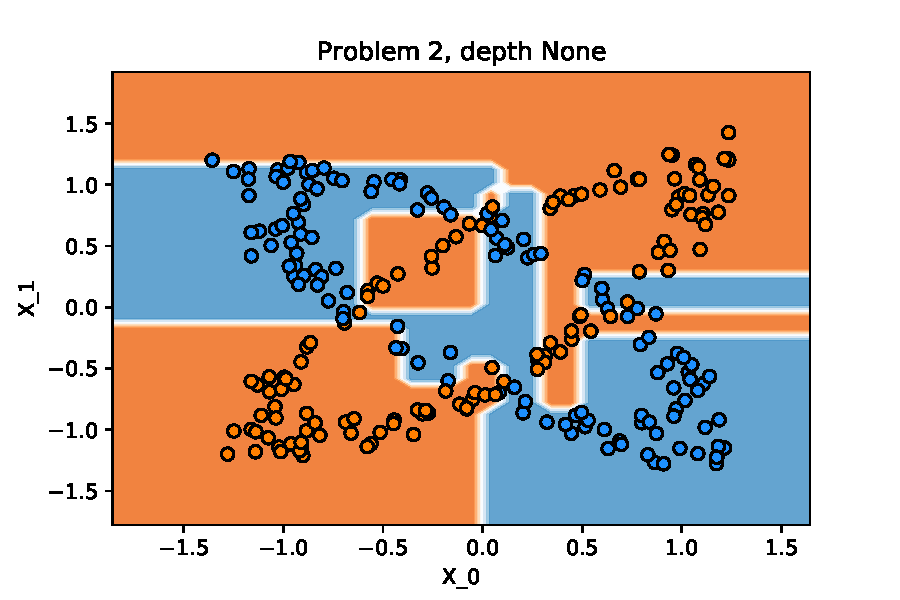
\includegraphics[width=\picwidth]{plots/dec_tree/p2_depthNone.pdf}}

  \caption{\label{boundary2}Decision boundaries problem 2}
\end{figure}
\FloatBarrier


\subsubsection{Overfitting and underfitting}

We assess :
\begin{enumerate}
\item Overfitting : if error rate on learning set is small compared to error rate on test set
\item Underfitting : if error rate on learning set is high
\end{enumerate}

So we have the following results (see tables \ref{overfitting1} and \ref{overfitting2}).

\begin{table}[h]
  \centering
	\begin{tabular}{rrrl}
	      \textbf{Depth} & \textbf{Learning set} & \textbf{Test set} & \textbf{Overfit} \\
	      \hline
	      1 & 26.8\% & 28.94\% & Underfit \\
2 & 5.6\% & 7.27\% & - \\
4 & 0.0\% & 0.66\% & - \\
8 & 0.0\% & 0.66\% & - \\
None & 0.0\% & 0.66\% & - \\
	\end{tabular}
  \caption{\label{overfitting1}Overfitting for problem 1}
\end{table}
	
\begin{table}[h]
  \centering
	\begin{tabular}{rrrl}
	      \textbf{Depth} & \textbf{Learning set} & \textbf{Test set} & \textbf{Overfit} \\
	      \hline
    1 & 47.2\% & 49.95\% & Underfit \\
2 & 45.2\% & 49.46\% & Underfit \\
4 & 15.2\% & 21.61\% & Underfit \\
8 & 5.2\% & 18.52\% & Overfit \\
None & 0.0\% & 14.85\% & Overfit \\

	\end{tabular}
  \caption{\label{overfitting2}Overfitting for problem 2}
\end{table}


\subsubsection{Model confidence}

For problem 1, the model becomes more confident for the obvious reason that it's boundary becomes more adapted to the problem.

For problem 2, it's less obvious. The model improves with depth up to depth 8 as it can split the space in distinct parts, that fits the greater number of point. However, at unconstraint depth, it can't sort out the intersection between the ellipses and tends to over fit (see above). So we'd say that although it's globally improving, it does become more instable locally.

	

\subsection{Test set accuracies over 5 generations}

We give the mean error rates and accomanying standard deviations for both problems at various depths. These are computed over 5 different sets of test data.

\begin{table}[h]
  \centering
\subfloat[Problem 1]{
	\begin{tabular}{rcr}
	      \textbf{Depth} & \textbf{Mean} & \textbf{Std dev}\\
	      \hline
	      1 & 28.75 & 0.24 \\
2 & 7.19 & 0.12 \\
4 & 0.61 & 0.05 \\
8 & 0.61 & 0.05 \\
None & 0.61 & 0.05 \\
	      
	\end{tabular}}
\subfloat[Problem 2]{
	\begin{tabular}{rcr}
	      \textbf{Depth} & \textbf{Mean} & \textbf{Std dev}\\
	      \hline
	      1 & 50.01 & 0.10 \\
2 & 49.82 & 0.32 \\
4 & 21.66 & 0.15 \\
8 & 18.56 & 0.49 \\
None & 14.76 & 0.22 \\
	\end{tabular}}
  \caption{\label{tbl_errors}Comparing mean and std dev. of error rates on both problems}
\end{table}

We conclude that problem 1's tree stabilizes from depth 4 on. For problem 2, the tree improves but continue to make a significant number of errors (see mean). Also, the standard deviation doesn't decrease with depth. Which means that the tree doesn't stabilize.

\subsection{Comparing problems one and two}

Considering the information above, we can say that the problem1 is much easier to deal with  a decision tree. The mean and std dev. of error rate converge towards 0 as depth increases, without much overfitting.
That's because the positions of the two set of points are clearly separated and their relative positions and shapes allow for a boundary to be built by sequentially dividing the space along orthogonal lines. 

Problem 2 is not good for a decision tree because the two sets of points overlap in some area. The mean never gets close to zero (even at  unconstrainted depth) and std dev. of error rate doesn't converge towards 0 as depth increases. Moreovoer overfitting occurs.

\section{K-nearest neighbors}


\subsection{Decision Boundaries}
\subsubsection{Boundaries}
	\begin{figure}[H]
		\centering
		
		\subfloat{   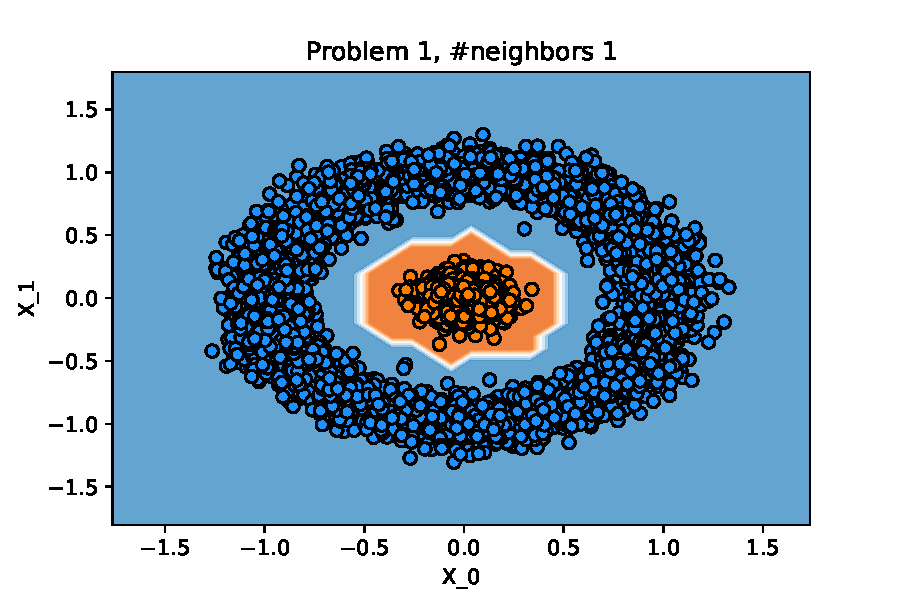
\includegraphics[width=\picwidth]{plots/neighbors/p1_neighbors1.pdf}}
		\subfloat{   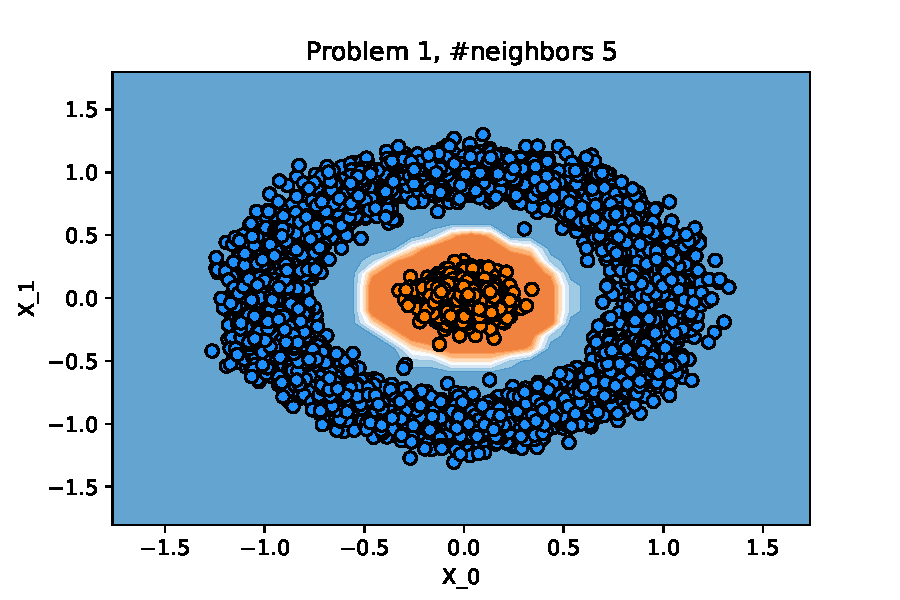
\includegraphics[width=\picwidth]{plots/neighbors/p1_neighbors5.pdf}}
		
		\subfloat{   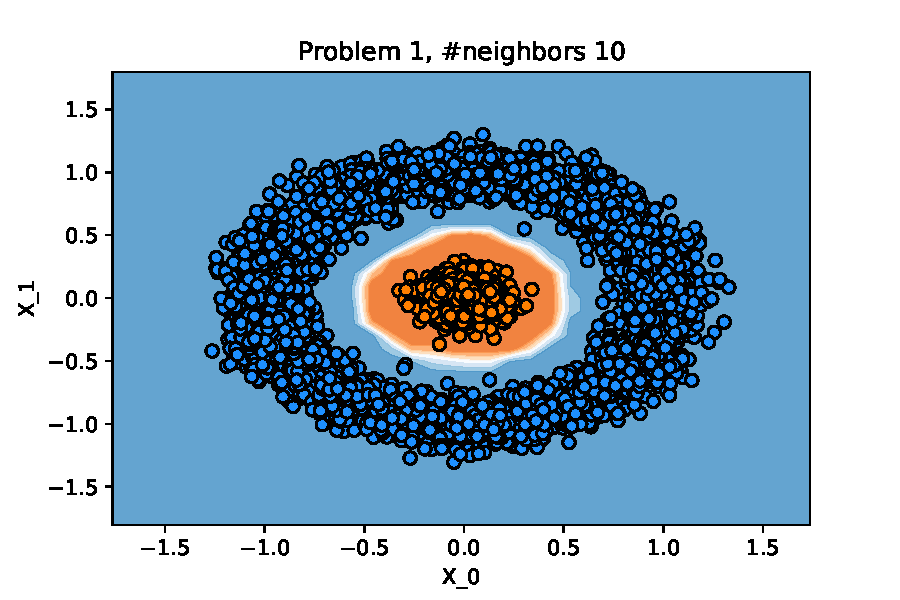
\includegraphics[width=\picwidth]{plots/neighbors/p1_neighbors10.pdf}}
		\subfloat{   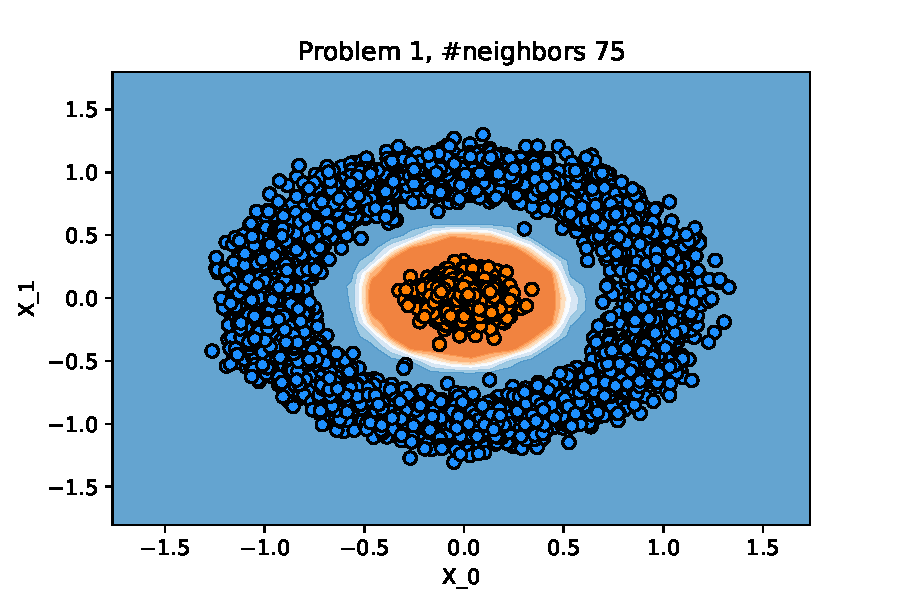
\includegraphics[width=\picwidth]{plots/neighbors/p1_neighbors75.pdf}}
		
		\subfloat{   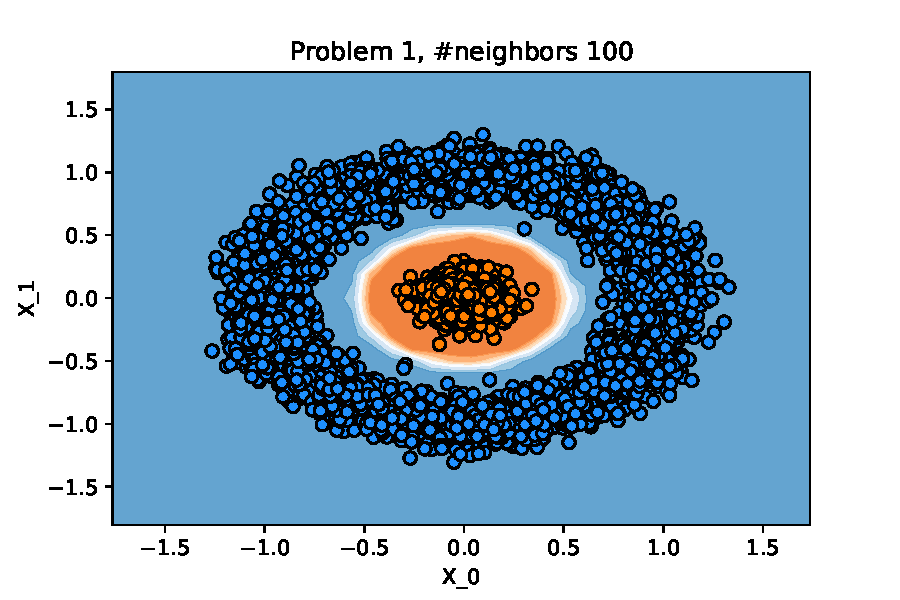
\includegraphics[width=\picwidth]{plots/neighbors/p1_neighbors100.pdf}}
		\subfloat{   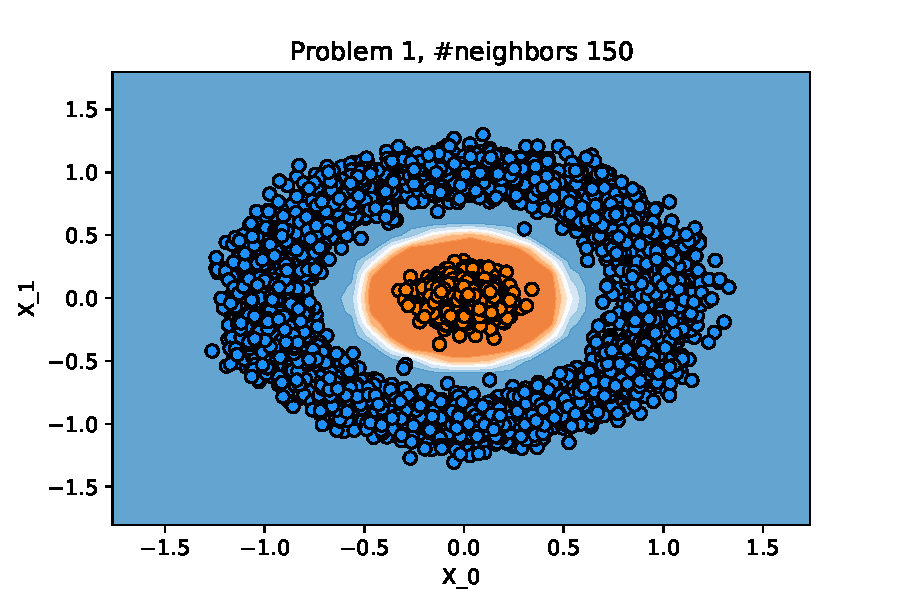
\includegraphics[width=\picwidth]{plots/neighbors/p1_neighbors150.pdf}}
		
		
		\caption{\label{boundary2.3p1}Decision boundaries problem 1}
	\end{figure}
	\begin{figure}[H]
		\centering
		
		\subfloat{   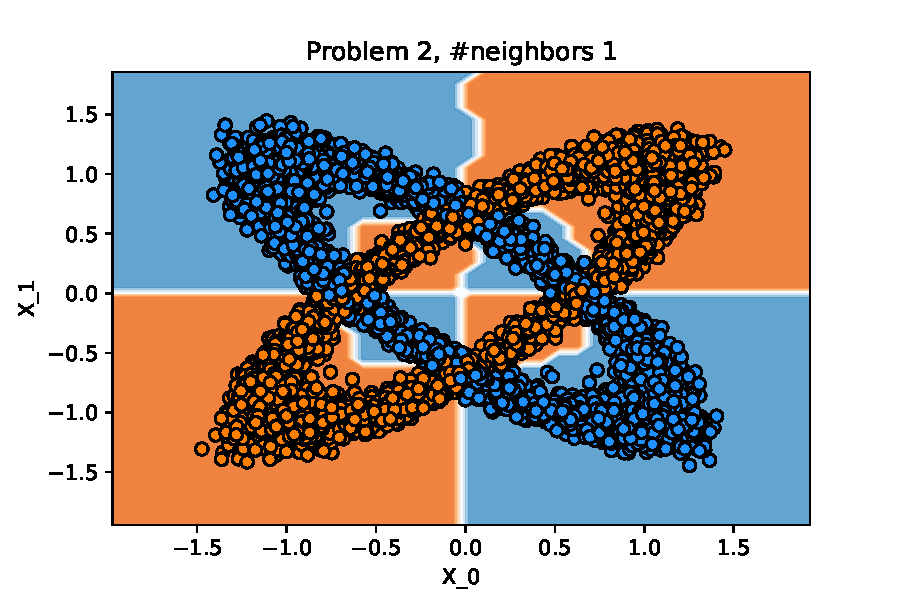
\includegraphics[width=\picwidth]{plots/neighbors/p2_neighbors1.pdf}}
		\subfloat{   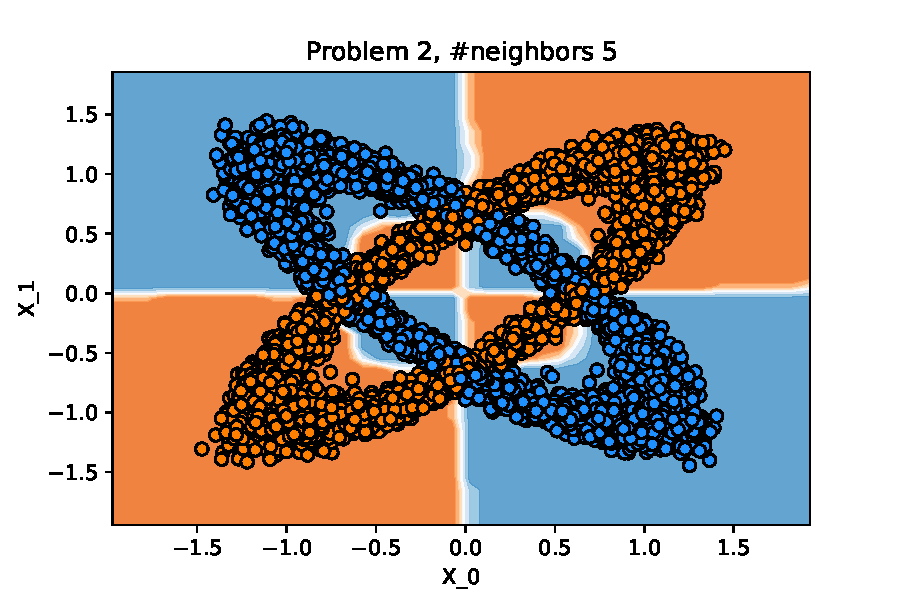
\includegraphics[width=\picwidth]{plots/neighbors/p2_neighbors5.pdf}}
		
		\subfloat{   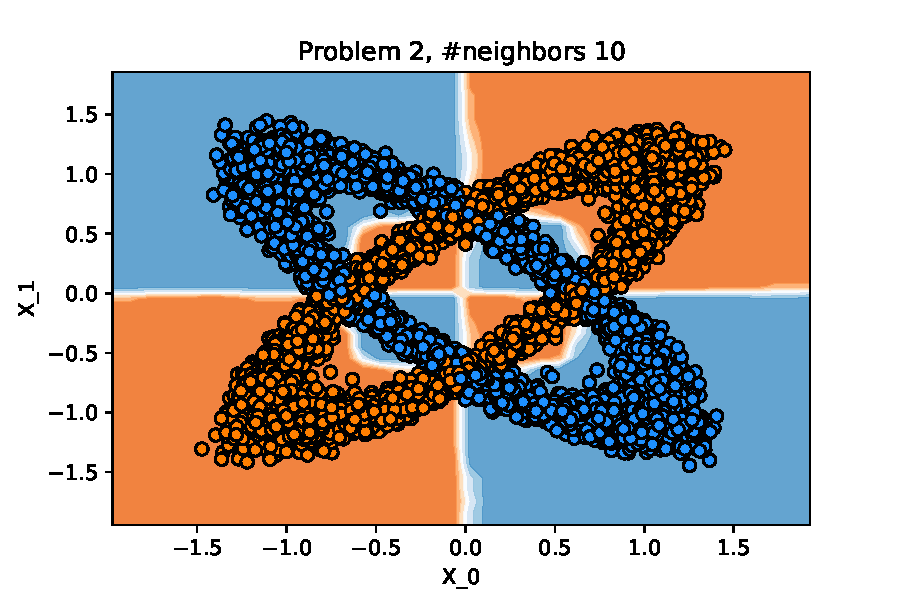
\includegraphics[width=\picwidth]{plots/neighbors/p2_neighbors10.pdf}}
		\subfloat{   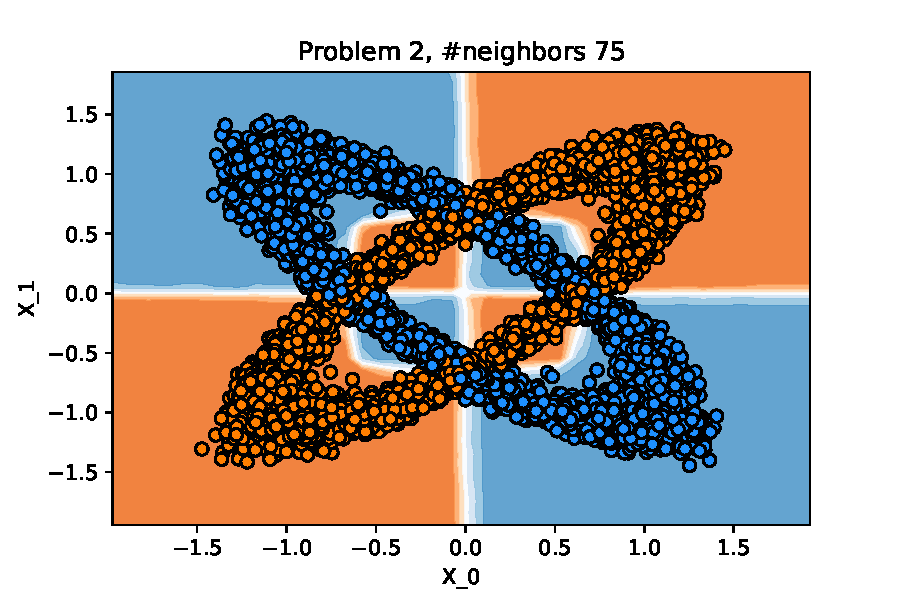
\includegraphics[width=\picwidth]{plots/neighbors/p2_neighbors75.pdf}}
		
		\subfloat{   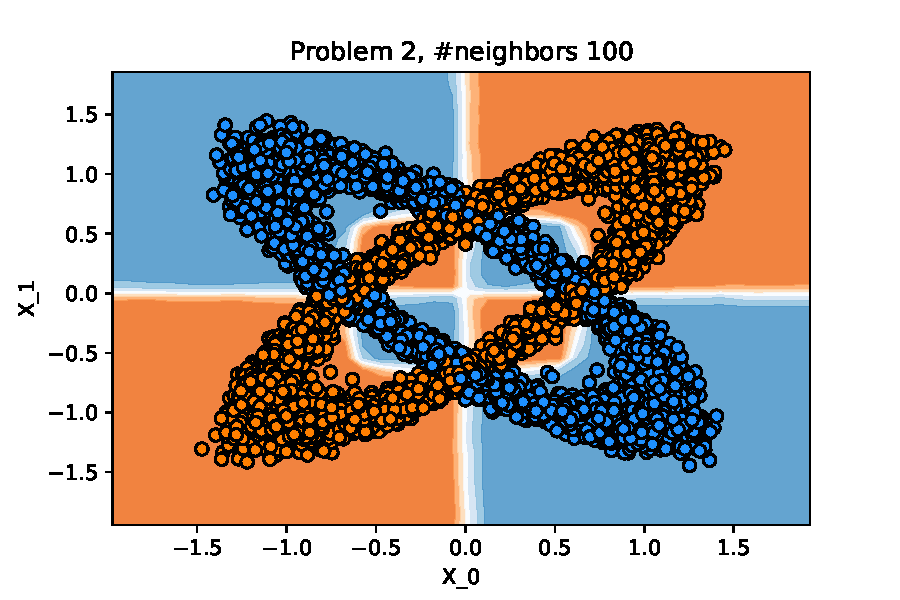
\includegraphics[width=\picwidth]{plots/neighbors/p2_neighbors100.pdf}}
		\subfloat{   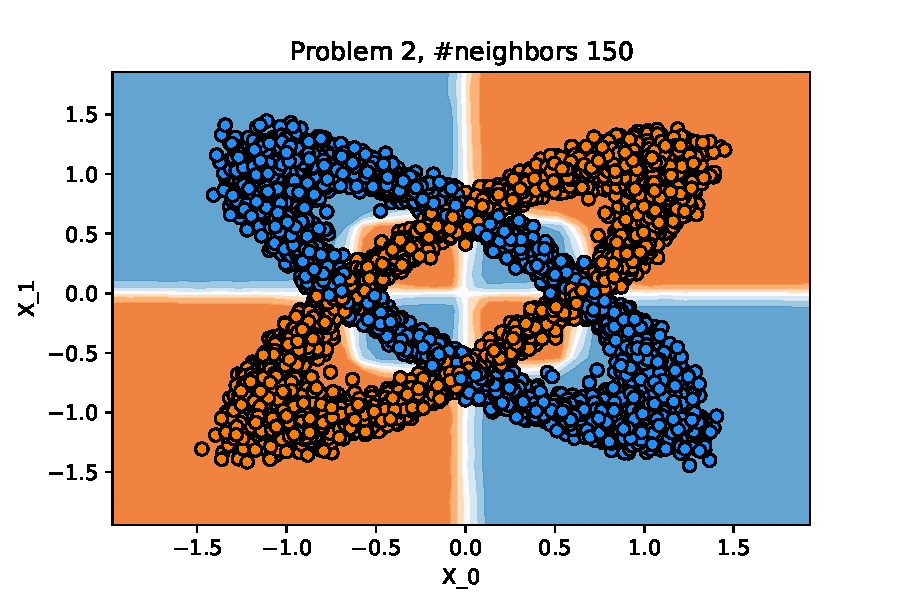
\includegraphics[width=\picwidth]{plots/neighbors/p2_neighbors150.pdf}}
		
		
		\caption{\label{boundary2.3p2}Decision boundaries problem 2}
		
	\end{figure}

\subsubsection{Comment}
The decision boundary for data set one seems to be quite good even for one neighbor. That is probably due to the fact that the two classes are neatly seperated in different regions. With a growing number of neighbors the boundary starts getting wider and therefore adding uncertainty to the classification. \\
The same is true for the second data set. The more neighbors are used the more uncertain the prediction becomes.

\subsection{Five-Fold Cross Validation}

\begin{enumerate}
	\item We began by partitioning the data set into five distinct subsets. That was achieved by randomly shuffling the original data and then choosing the first 2000 elements in upcoming order for every subset. For every possible number of neighbors we then did the following procedure:
	\begin{itemize}
		\item Choose one subset
		\item Learn the model on the other subsets
		\item Compute the accuracy of the predictions on chosen subset
		\item Iterate over all subsets and then compute the mean of the accuracies.
	\end{itemize}
	Afterwards we selected the number of neighbors that achieved the highest mean accuracy over the five subsets.
	\item
	The optimal value for the neighbors is 5 and the mean of the accuracies 16.84\%. Just by looking at the plotted decision boundaries for the learning set in section 2.1 we would have expected to see 1 as the optimal value. 
\end{enumerate}

\subsection{Optimal Value of Neighbors with respect to LS Size}
\subsubsection{Plots}
		\begin{figure}[H]
		\centering
		
		\subfloat{   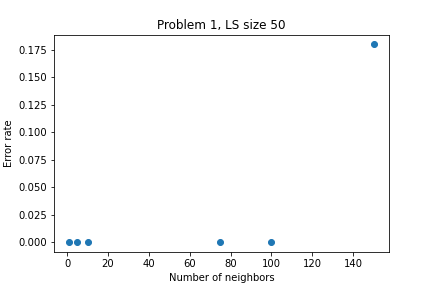
\includegraphics[width=\picwidth]{plots/neighbors/2.2/p1_neighbors150_ls50.png}}
		\subfloat{   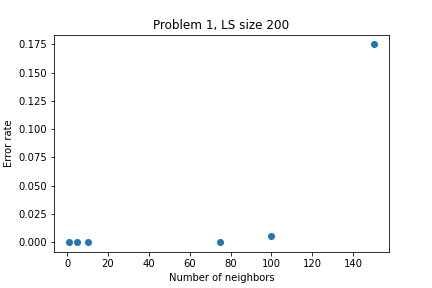
\includegraphics[width=\picwidth]{plots/neighbors/2.2/p1_neighbors150_ls200.png}} \\
			\subfloat{   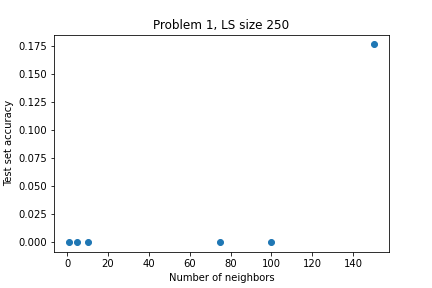
\includegraphics[width=\picwidth]{plots/neighbors/2.2/p1_neighbors150_ls250.png}}
				\subfloat{   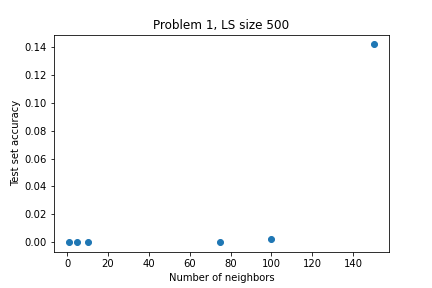
\includegraphics[width=\picwidth]{plots/neighbors/2.2/p1_neighbors150_ls500.png}}
				
		
		\caption{\label{acc2.3p1}Test Set Accuracies Problem 1}
		
	\end{figure}
	\begin{figure}[H]
	\centering
	\subfloat{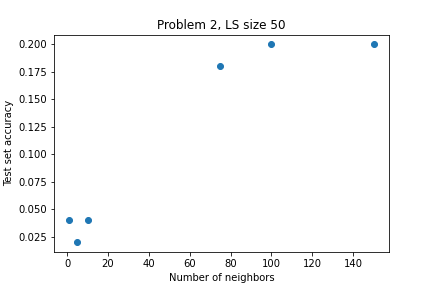
\includegraphics[width=\picwidth]{plots/neighbors/2.2/p2_neighbors150_ls50.png}}
	\subfloat{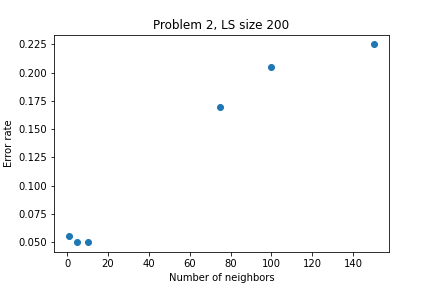
\includegraphics[width=\picwidth]{plots/neighbors/2.2/p2_neighbors150_ls200.png}} \\
	\subfloat{   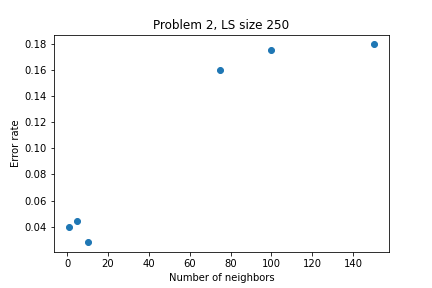
\includegraphics[width=\picwidth]{plots/neighbors/2.2/p2_neighbors150_ls250.png}}
	\subfloat{   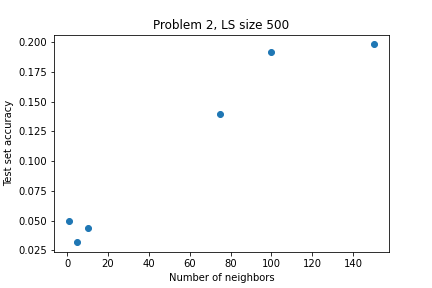
\includegraphics[width=\picwidth]{plots/neighbors/2.2/p2_neighbors150_ls500.png}}
	
	\caption{\label{acc2.3p2}Test Set Accuracies Problem 2}
	
\end{figure}
\begin{figure}[H]
	\centering
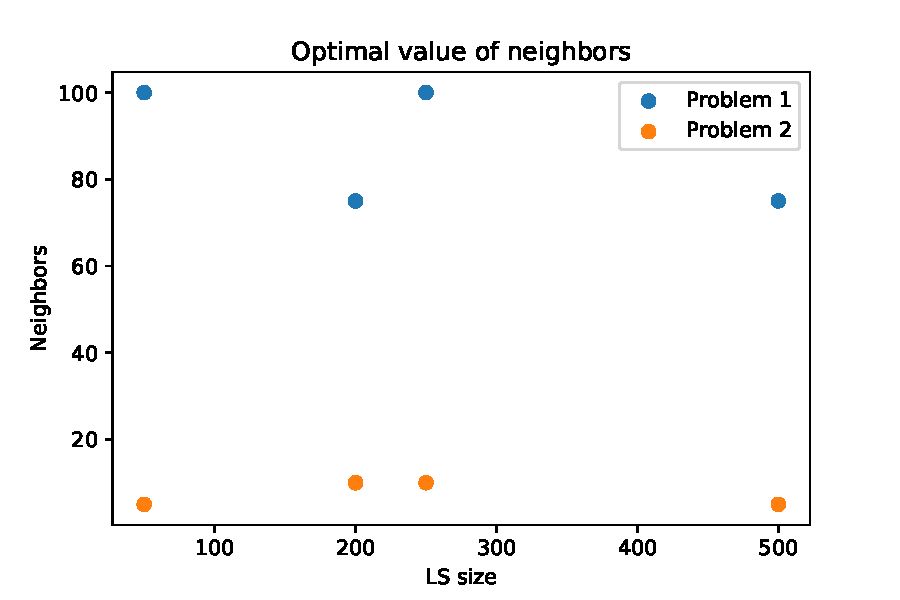
\includegraphics[width=\picwidth]{plots/neighbors/2.3/optimal_values.pdf}
	\caption{\label{acc2.3p2}Optimal number of neighbors}
	
\end{figure}
\subsubsection{Comment}
For the first data set, regardless of the size of the learning set, we observe that one neighbor produces the best accuracy. As the number of neighbors increases, the accuracy slightly increases. However, when 150 neighbors are used the error rate is considerably higher than in the other cases. \\
For the first three choices of the neighbors, the second data set is fitted quite nicely. The optimal number of neighbors depends on the actual size of the learning set, but it is always found among the three smallest number of neighbors. Starting from 75 neighbors, the error rate rises drastically and peaks at 150 neighbors.
\subsection{Last Question}
We don't think using cross validation is a good strategy for data set one because the achieved error rate among the three best choices does not differ by much. Therefore you can almost arbitrarily choose one of the three lowest numbers of neighbors and get an optimal result. \\
In the case of data set 2, however, a cv approach could be used to find the best number among the three smallest. It could be a good strategy here since the error rates for the three lowest number of neighbors are distinctly different and so can be fine tuned. 
% ==============================================================================

\end{document}